\textbf{9.1.} 一长螺线管的自感为 $L$ ，当它的导线中通有电流 $I$ 时，试证明它所储藏的能量为 $W_{m} = \frac{1}{2} LI^{2}$ ；设这能量储存在磁场中，磁场是均匀的，试证明：磁场能量密度（即单位体积内的磁场能量）为 $W_{m} = \frac{1}{2} H \cdot B$ .

\vfill

\textbf{9.2.} 一螺线管长为 $l = 300\mathrm{mm}$ , 横截面的直径为 $d = 15\mathrm{mm}$ , 由表面绝缘的细导线密绕而成, 共有 N=2500 匝. 当导线中通有电流 I=2.0A 时, 试求管中心的磁场强度 H、磁感强度 B 和磁场能量密度 $w_{m}$ 等的值.

\vfill

\newpage

\textbf{9.3.} 一螺线管长 $30\mathrm{cm}$ , 横截面的直径为 $12\mathrm{cm}$ , 由 600 匝表面绝缘的细导线密绕而成. 管内是空气. 当它的导线中通有 $1.0\mathrm{A}$ 的电流时, 试分别求管中心和管口轴线上的磁场能量密度.

\vfill

\textbf{9.4.} 半径为 $a$ 的无限长直圆柱面均匀带电, 单位面积的电荷量为 $\sigma$ . 当这圆柱面以匀角速度 $\omega$ 绕它的几何轴旋转时, 试求圆柱内单位长度的磁场能量.

\vfill

\newpage

\textbf{9.5.} 电荷量 Q 均匀地分布在半径为 a 的球面上, 当这球面以匀角速度 $\omega$ 绕它的一个固定直径旋转时, 试求球内的磁场能量.

\vfill

\textbf{9.6.} 一螺绕环由外表绝缘的导线在硬纸壳上绕 $N$ 匝而成，横截面积为 $a \times b$ ，内半径为 $R$ ，外半径为 $R + b$ ，它的一半如图9.6所示。当导线内的电流为 $I$ 时，试求这螺绕环体内的磁场能量。

\vfill

\newpage

\textbf{9.7.} 一同轴电缆由很长的直导线和套在它外面的同轴导体圆筒构成,导线的半径为 a, 圆筒的半径为 b, 圆筒的厚度可略去不计.电流 I 由圆筒流去,由导线流回, I 在导线和圆筒的横截面上,都是均匀分布的.试求:(1)离轴线为 r 处的磁场能量密度 $w_{m}$ ;(2)这电缆长为 l 的一段所储存的磁场能量 $W_{m}$ ;(3)当 a = 1.0mm, b = 7.0mm, l = 1.00m 和 I = 100A 时 $W_{m}$ 的值.

\vfill

\textbf{9.8.} 一同轴传输线由很长的直导线和套在它外面的同轴导体圆管构成,导线的半径为 a,圆管的内半径为 b,外半径为 c.电流 I 由圆管流去,由导线流回;I 在它们的横截面上都是均匀分布的.(1)试求下列四处一米长的磁场能量:(i)导线内；(ii)导线和圆管之间；(iii)圆管本身内；(iv)圆管外.(2)当 $a = 1.0\mathrm{mm},b =$ $4.0\mathrm{mm},c = 5.0\mathrm{mm},I = 10\mathrm{A}$ 时，试计算上述各处磁场能量的值.磁场能量主要分布在什么地方？

\vfill

\newpage

\textbf{9.9.} 一同轴电缆由半径为 $a$ 的长直导线和与它共轴的导体薄圆筒构成, 圆筒的半径为 $b$ , 如图 9.9 所示. 导线与圆筒间充满电容率为 $\varepsilon$ 、磁导率为 $\mu$ 的均匀介质. 当电缆的一端接上负载电阻 $R$ , 另一端加上电势差时, 试证明: 如果 $R = \frac{1}{2\pi} \sqrt{\frac{\mu}{\varepsilon}} \ln \frac{b}{a}$ , 则导线与圆筒间的电场能量等于磁场能量.
\begin{center}
    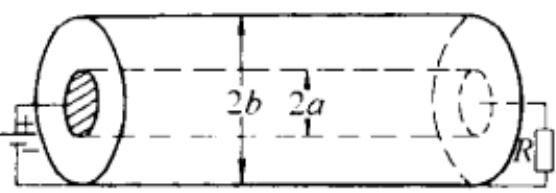
\includegraphics[width=0.5\linewidth]{figures/fig_9_9.jpg}
\end{center}

\vfill

\textbf{9.10.} 两无限长直薄圆筒共轴, 半径分别为 $R_{1}$ 和 $R_{2}$ , 载有大小相等而方向相反的电流 $I, I$ 平行于轴线流动, 并均匀分布在筒面上. 两筒间充满磁导率为 $\mu$ 的均匀介质. 试求下列各处长为 $l$ 一段的磁场能量: (1) 内筒内; (2) 两筒间; (3) 外筒外.

\vfill

\newpage

\textbf{9.11.} 一条很长的直导线, 半径为 $R$ , 载有电流 $I, I$ 均匀分布在它的横截面上. 导线外有一层厚为 $h$ 的绝缘皮. (1) 试求这导线里单长度的磁场能量; (2) 在这导线里取一共轴的小圆柱体, 其半径为 $\frac{R}{2}$ , 试求这小圆柱里单位长度的磁场能量; (3) 试求外皮里单位长度的磁场能量.

\vfill

\textbf{9.12.} 一铁环上绕有 N = 500 匝外皮绝缘的导线，当导线中的电流为 I = 2.0A 时，穿过铁环横截面的磁通量为 $3.0 \times 10^{-3} ~Wb$ . 试求铁环内的磁场能量.

\vfill

\newpage

\textbf{9.13.} 一起重用的电磁铁由 U 形轭铁和铁块构成, 如图 9.13 所示. 设轭铁每个极的面积都是 $S = 1.5 \times 10^{-2} \mathrm{~m}^2$ , 磁通量都是 $\Phi = 1.5 \times 10^{-2} \mathrm{Wb}$ . 试求这电磁铁的起重力(包括铁块的重量在内).

\vfill

\textbf{9.14.} 一导线弯成半径为 $R = 5.0\mathrm{cm}$ 的圆形，当其中载有 $I = 100\mathrm{A}$ 的电流时，试求圆心的磁场能量密度 $\omega_{m}$ .

\vfill

\newpage

\textbf{9.15.} 按照玻尔理论,氢原子处在基态时,它的电子沿半径为 $a = 5.29 \times 10^{-11}$ m 的圆轨道绕氢核(质子)运动.已知电子的质量为 $m = 9.11 \times 10^{-31}$ kg,电荷量为 $e = -1.60 \times 10^{-19}$ C.试求电子的这种运动在轨道中心产生的磁场能量密度.

\vfill

\textbf{9.16.} 半径都是 R 的两共轴圆线圈, 载有大小和方向都相同的电流 I, 它们间的距离等于半径 R (亥姆霍兹线圈). 试求轴线上离两线圈都相等处的磁场能量密度.

\vfill

\newpage

\textbf{9.17.} 对于一个电源来说, 若电流的方向与它的电动势方向(非静电力的方向)相同, 即从它的正极出发, 经外电路回到负极, 如图 9.17(1) 所示, 则这时电源对外供电, 因而它的能量减少; 若电流的方向与电动势方向(非静电力的方向)相反, 则电源的能量便增多. 上述结论对于载有电流 I 的自感线圈 L 来说, 是否正确, 试就图 9.17(3) 中 (i) $\frac{\mathrm{d}I}{\mathrm{d}t} < 0$ , (ii) $\frac{\mathrm{d}I}{\mathrm{d}t} = 0$ 和 (iii) $\frac{\mathrm{d}I}{\mathrm{d}t} > 0$ 三种情况, 分别加以说明.

\vfill

\textbf{9.18.} 一线圈的自感为 $L = 5.0\mathrm{H}$ , 电阻为 $R = 20\Omega$ , 将 $U = 100\mathrm{V}$ 的不变电压加到它的两端. (1) 试求电流达到最大值 $I_0 = \frac{U}{R}$ 时, 线圈所储存的磁能 $W_m$ ; (2) 从线圈两端加上电压开始算起, 试问经过多长时间, 线圈所储存的能量达到 $W_m / 2$ ? (3) 线圈所储存的磁能从 $W_m / 2$ 增加到 $0.99W_m$ , 需要多长时间?

$$
\text {   【解】   } (1) W _ {m} = \frac {1}{2} L I _ {0} ^ {2} = \frac {1}{2} L \left(\frac {U}{R}\right) ^ {2} = \frac {1}{2} \times 5. 0 \times \left(\frac {1 0 0}{2 0}\right) ^ {2} = 6 3 (\mathrm{J})
$$

(2)加上电压 U 后,电路方程为

(1)

$$
L \frac {\mathrm{d} I}{\mathrm{d} t} + R I = U\tag{2}
$$

利用初始条件 t=0 时, I=0, 解式(2)得

$$
I = \frac {U}{R} (1 - \mathrm{e} ^ {- \frac {R}{L} t})\tag{3}
$$

当 $L$ 储存的能量为

$$
\frac {1}{2} L I ^ {2} = \frac {1}{2} W _ {m} = \frac {1}{4} L I _ {0} ^ {2}\tag{4}
$$

时

$$
I = \frac {I _ {0}}{\sqrt {2}} = \frac {1}{\sqrt {2}} \frac {U}{R}\tag{5}
$$

代入式(3)得

$$
1 - \mathrm{e} ^ {- \frac {R}{L} t} = \frac {1}{\sqrt {2}}\tag{6}
$$

解得

$$
t = \frac {L}{R} \ln \sqrt {2} (\sqrt {2} + 1) = \frac {5 . 0}{2 0} \times \ln (1. 4 1 4 \times 2. 4 1 4) = 0. 3 1 (\mathrm{s})\tag{7}
$$

(3) 当 L 储存的能量为 $0.99 W_{m}$ 时，

$$
\frac {1}{2} L I ^ {2} = 0. 9 9 \times \frac {1}{2} L I _ {0} ^ {2}\tag{8}
$$

代入式(3)得

$$
1 - \mathrm{e} ^ {- \frac {R}{L} t} = \sqrt {\frac {9 9}{1 0 0}} = \frac {3 \sqrt {1 1}}{1 0}\tag{9}
$$

解得

$$
t ^ {\prime} = \frac {5 . 0}{2 0} \ln \left(\frac {1 0}{1 0 - 3 \sqrt {1 1}}\right) = 1. 3 (\mathrm{s})\tag{10}
$$

故得所求的时间为

$$
\Delta t = t ^ {\prime} - t = 1. 3 - 0. 3 1 = 1. 0 (\mathrm{s})\tag{11}
$$

\vfill

\newpage

\textbf{9.19.} 一电路如图 9.19(1), L 和 R 串联, 将 K 接到 a, 使电流流过 L 和 R. 然后将 K 迅速拨向 b, 在 t=0 时刻, K 接到 b, 这时 L 和 R 中的电流为 $I_{0}$ . (1) 试求此后电流与时间 t 的关系; (2) 试证明: L 所储藏的磁能将全部化为 R 上消耗的焦耳热.


图9.19(1)
图9.19(2)
\begin{center}
    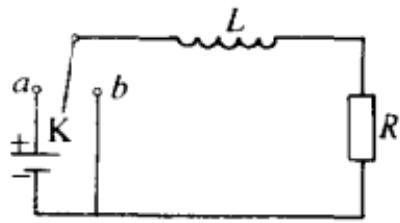
\includegraphics[width=0.5\linewidth]{figures/fig_9_19_1.jpg}
\end{center}
\begin{center}
    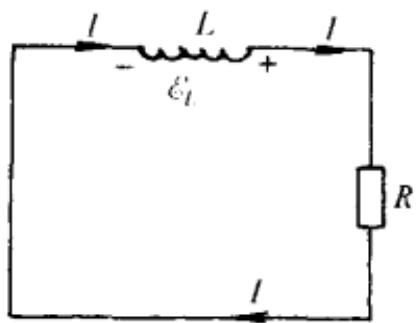
\includegraphics[width=0.5\linewidth]{figures/fig_9_19_2.jpg}
\end{center}

\vfill

\textbf{9.20.} 如图 9.20(1)，一电容为 C 的电容器蓄有电荷量 $Q_{0}$ ，在 t=0 时刻接通 K，使它经过自感为 L 的线圈放电。试求：(1)L 内的磁场能量第一次等于 C 内电场能量的时刻 $t_{1}$ ; (2)L 内的磁场能量第二次达到极大值的时刻 $t_{2}$ 。

图9.20(1)

图9.20(2)
\begin{center}
    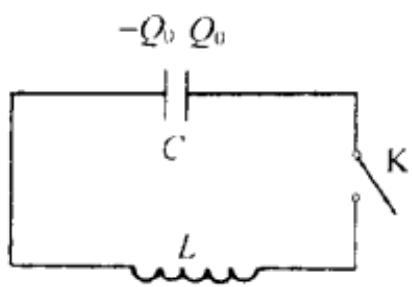
\includegraphics[width=0.5\linewidth]{figures/fig_9_20_1.jpg}
\end{center}
\begin{center}
    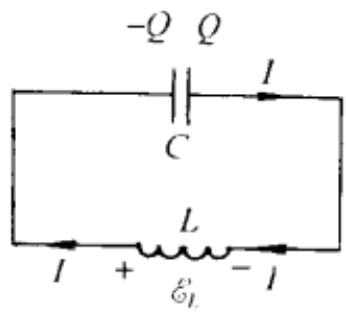
\includegraphics[width=0.5\linewidth]{figures/fig_9_20_2.jpg}
\end{center}

\vfill

\newpage

\textbf{9.21.} 一电路如图 9.21, 已知电阻 $R = 5.0\Omega$ , 电感 $L = 0.60\mathrm{H}$ , 电源的电动势 $\varepsilon = 12\mathrm{V}$ , 内阻 $r = 1.0\Omega$ . 试求接通电键 S 后 $0.10\mathrm{s}$ 时, (1) 电阻 $R$ 消耗的功率; (2) 电感 $L$ 的磁能增加率; (3) 电源的输出功率.

\vfill

\textbf{9.22.} 一电路如图 9.22, 其中 E、r、R 和 L 均为已知.
(1)试求 K 接通后,电流达到稳定值时,L 所储存的能量;
(2)这能量以什么形式储存在 L 中? (3)电流达到稳定值后断开 K,试求 L 所储存的能量随时间的变化率;(4)试证明: K 断开后,R 放出的焦耳热等于 L 所储存的能量.
\begin{center}
    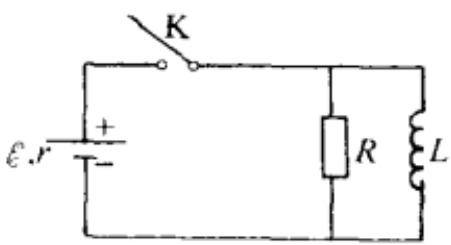
\includegraphics[width=0.5\linewidth]{figures/fig_9_22.jpg}
\end{center}

\vfill

\newpage

\textbf{9.23.} 任何两个线圈1和2,试用磁场能量的方法证明:1对2的互感 $M_{21}$ 等于2对1的互感 $M_{12}$ .

\vfill

\textbf{9.24.} 根据实验,在北纬 $40^{\circ}$ 某处,地面的电场强度为 300V/m,磁感强度为 $5.49 \times 10^{-5}T$ .试分别求该处的磁场能量密度和电场能量密度以及它们的比值.

\vfill

\newpage

\textbf{9.25.} 目前在实验里,利用先进技术,在空气中产生 B=1.0T 的磁场并不困难.(1)试求这磁场的能量密度;(2)要想产生电场能量密度等于这个值的电场,试问电场强度 E 的值应为多少?这在实验上容易实现吗?

\vfill

\textbf{9.26.} 目前在实验室里产生 $E = 10^{5} V/m$ 的电场或 $B = 10^{4} Gs$ 的磁场是不难做到的. 今在边长为 10cm 的立方体空间内产生上述两种均匀场, 试问所需的能量各为多少? 磁场能量是电场能量的多少倍?

\vfill

\newpage

\textbf{9.27.} 用超导材料制成的螺线管, 可以获得 15 特斯拉的强磁场, 试求这磁场的能量密度.

\vfill

\textbf{9.28.} 设一带电粒子是半径为 $R$ 的圆球, 所带的电荷量 $q$ 均匀地分布在球面上. 当这粒子以匀速 $\pmb{v}(v \ll c)$ 运动时, 在它外面的空间里离球心 $O$ 为 $\pmb{r}$ (图9.28) 处产生的磁场强度为

$$
\boldsymbol {H} = \frac {q \boldsymbol {v} \times \boldsymbol {r}}{4 \pi r ^ {3}}
$$

试求这磁场的总能量.

\vfill

\newpage

\textbf{9.29.} 试由电磁学的基本关系推导出下列一些量的单位: $E, D, \varepsilon_0, H, B, \mu_0, E \cdot D, H \cdot B$ 和 $E \times H$ .

\vfill
